\documentclass{scrartcl}

%Aus dem LaTex Template der Universit�t Stuttgart
%------------------------------------------------
\usepackage[utf8]{inputenc}
\usepackage[T1]{fontenc}
\usepackage[sfdefault]{ClearSans} %% option 'sfdefault' activates Clear Sans as the default text font
\usepackage{cmap}
\usepackage[ngerman]{babel}
\usepackage{graphicx}
\usepackage[pdftex,hyperref,dvipsnames]{xcolor}
\usepackage{listings}
\usepackage[a4paper,lmargin={2cm},rmargin={2cm},tmargin={3.5cm},bmargin = {2.5cm},headheight = {4cm}]{geometry}
\usepackage{amsmath,amssymb,amstext,amsthm}
\usepackage[lined,algonl,boxed]{algorithm2e}
\usepackage{tikz}
\usepackage{hyperref}
\usepackage{url}
\usepackage[inline]{enumitem} % Erm�glicht �ndern der enum Item Zahlen
\usepackage[headsepline]{scrpage2} 
\usepackage{algorithmic} % F�r Pseudocode
\usepackage{ marvosym } % f�r Pfeil(e)
\usepackage{booktabs} % F�r die sch�neren Booktabs-Tabellen
\usepackage{tikz}
\usepackage{pdfpages}
\usepackage{blindtext}
\usepackage{scrextend}
\usepackage{pdfpages}
\usepackage{natbib} % Yannis hat das importiert; TODO: nachfragen, zu was das gut ist
\pagestyle{scrheadings} 
\usetikzlibrary{automata,positioning}

\begin{document}
	%%% Vorgegebenes Deckblatt %%%
	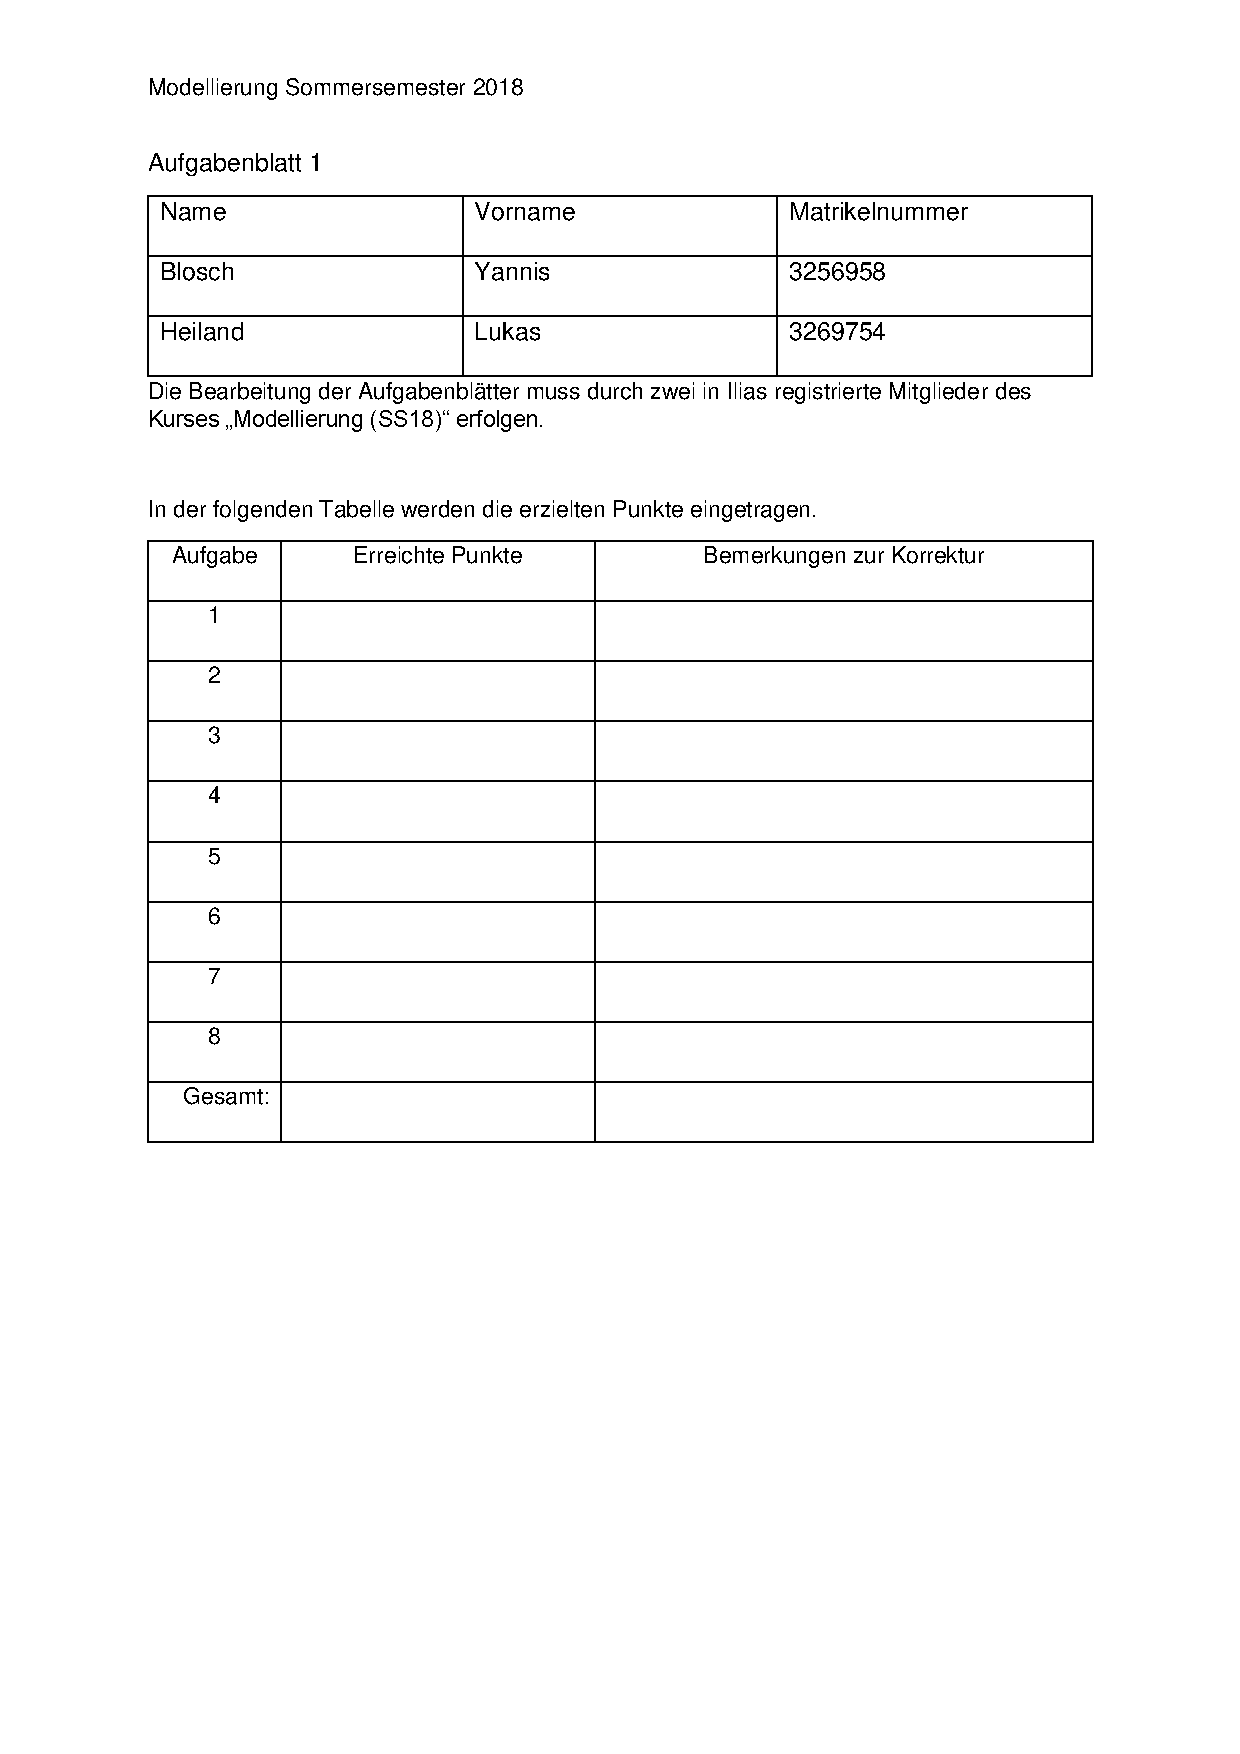
\includepdf{deckblatt.pdf}
	%%% format and header %%%
	% Counter für das Blatt und die Aufgabennummer.
% Ersetze die Nummer des Übungsblattes und die Nummer der Aufgabe
% den Anforderungen entsprechend.
% Beachte:
% \setcounter{countername}{number}: Legt den Wert des Counters fest
% \stepcounter{countername}: Erhöht den Wert des Counters um 1.
\newcounter{sheetnr}
\setcounter{sheetnr}{1} % Nummer des Übungsblattes
\newcounter{exnum}
\setcounter{exnum}{1} % Nummer der Aufgabe

% Befehl für die Aufgabentitel
\newcommand{\exercise}[1]{\section*{Aufgabe \theexnum\stepcounter{exnum} #1}} % Befehl für Aufgabentitel

% Formatierung der Kopfzeile
% \ohead: Setzt rechten Teil der Kopfzeile mit
% Namen und Matrikelnummern aller Bearbeiter
\ohead{Yannis Blosch (3256958)\\
Lukas Heiland (3269754)}
% \chead{} kann mittleren Kopfzeilen Teil sezten
% \ihead: Setzt linken Teil der Kopfzeile mit
% Modulnamen, Semester und Übungsblattnummer
\ihead{Modellierung\\
Sommersemester 2018\\
Blatt \thesheetnr}

	
	\section*{Aufgabe 6.1}
		\paragraph*{a.}
			\begin{itemize}
				\item Elementnamen d"urfen nicht mit den Buchstaben $ xml $ beginnen
				\item Elementnamen d"urfen keine Leerzeichen enthalten
				\item 
			\end{itemize}
		
		\paragraph*{b.}
			\begin{itemize}
				\item Die Modell-ID vom ersten Fahrzeug-Element ist falsch, ein Leerzeichen im Namen ist unzulässig
				\item Drittletzte Zeile: im schließenden $ <Modell> $-Tag fehlt ein  / (bzw. es ist demnach kein schließendes Tag)
				\item Erstes Fahrzeug-Element: Farbe erst groß, dann klein geschrieben
				\item Wert des $ einheit-$Attributs nicht in Anf"uhrungszeichen 
				\item Das zweite $ Fahrzeug $ hat kein schließendes Tag	
			\end{itemize}
	
	\section*{Aufgabe 6.2}
		
	\begin{verbatim}
		<?xml version="1.0" encoding="UTF-8"?>
		  <xs:schema xmlns:xs="http://www.w3.org/2001/XMLSchema">
		   <!-- Pruefungstyp -->
		   <xs:complexType name="Pruefung">
		
		    <xs:sequence>
		      <!-- Pruefungsnummer -->
		      <xs:element name="Nummer" type="xs:nonNegativeInteger" />
		
		      <!-- Titel der Pruefung -->
		      <xs:element name="Titel" type="xs:string" />
		
		      <!-- Art der Prüfung (schriftl./mündl.) -->
		      <xs:element name="Art">
		 
		        <xs:simpleType>
		         <xs:restriction base="xs:string">
		           <xs:enumeration value="muendlich"/>
		           <xs:enumeration value="schriftlich"/>
		         </xs:restriction>
		
		        </xs:simpleType>
		       </xs:element>
		      </xs:sequence>
		    </xs:complexType>
		
		
		
		    <!-- Studententyp -->
		    <xs:complexType name="Student">
		    
		     <xs:sequence>
		     
		       <!-- Name des Studenten -->
		       <xs:element name="Name" type="xs:string"/>
		
		       <xs:element name="Matrikelnr">
		          <xs:simpleType>
		            <xs:restriction base="xs:nonNegativeInteger">
		              <xs:pattern value="\d{6}"></xs:pattern>
		            </xs:restriction>
		          </xs:simpleType>
		       </xs:element>
		       
		       <!-- Adresse -->
		       <xs:sequence>
		          <xs:element name="Strasse" type="xs:string"/>
		          <xs:element name="Hausnummer" type="xs:nonNegativeInteger"/>
		          <xs:element name="PLZ" type="xs:nonNegativeInteger"/>
		          <xs:element name="Stadt" type="xs:string"/>
	     	   </xs:sequence>
		    </xs:sequence>
		   </xs:complexType>
		
		
		
		
		   <!-- "teilnehmen"-Relation -->
		   <xs:complexType name="teilnehmen">
		    <!-- Student minOccurs=unbounded -->
		    <!-- Pruefung minOccurs=1 maxOccurs=unbounded -->
		  </xs:complexType>
		</xs:schema>
	\end{verbatim}
		
	\pagebreak
	\section*{Aufgabe 6.3}.
		\begin{figure}[h]
			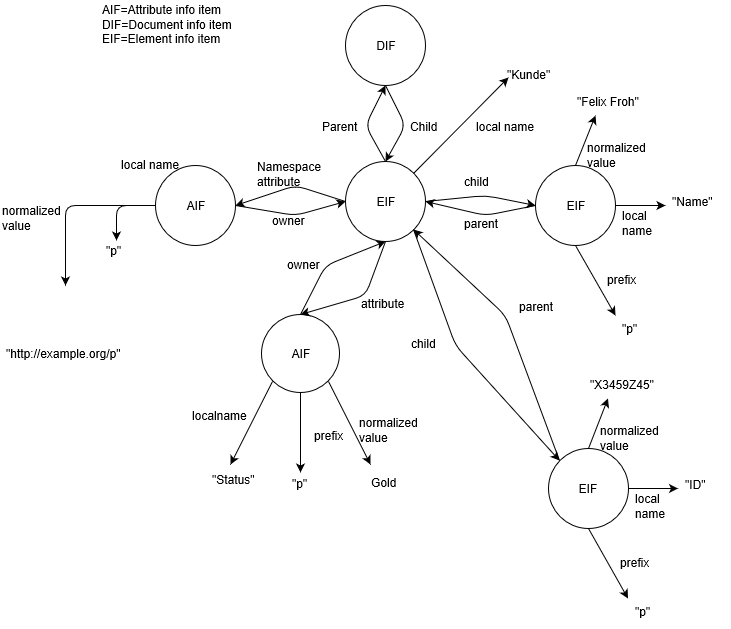
\includegraphics[scale=0.75]{aufgabe_6_3.png}
		\end{figure}
		
\end{document}